\section{Method}

\subsection{Overview}
\methodname is an image-to-video (I2V) diffusion generative model, which applies both an input image and a 3D tracking video as conditions for controllable video generation. In the following, we first review the backend I2V video diffusion model in Sec.~\ref{sec:dit}. Then, we discuss the definition of the 3D tracking video and how to inject the 3D tracking video into the generation process as a condition in Sec.~\ref{sec:tracking}. Finally, in Sec.~\ref{sec:control}, we discuss how to apply \methodname in various types of video generation control.

\subsection{Backend video diffusion model}
\label{sec:dit}

\methodname is finetuned from the CogVideoX~\cite{yang2024cogvideox} model that is a transformer-based video diffusion model~\cite{peebles2023scalable} operating on a latent space. 
Specifically, as shown in Figure~\ref{fig:pipe} (d), we adopt the I2V CogVideoX model as the base model, which takes an image $\mathbf{I}\in \mathbb{R}^{H\times W \times 3}$ as input and generate a video $\mathbf{V} \in \mathbb{R}^{T\times H\times W\times 3}$. The generated video $\mathbf{V}$ has $T$ frames with the same image size of width $W$ height $H$ as the input image. The input image $\mathbf{I}$ is first padded with zeros to get an input condition video with the same size $T\times H\times W \times 3$ as the target video. Then, a VAE encoder is applied to the padded condition video to get a latent vector of size $\frac{T}{4}\times \frac{H}{8}\times \frac{W}{8}\times 16$, which is concatenated with a noise of the same size. A diffusion transformer (DiT) \cite{peebles2023scalablediffusionmodelstransformers} is iteratively used to denoise the noise latent for a predefined number of steps and the output denoised latent is processed by a VAE decoder to get the video $\mathbf{V}$. In the following, we discuss how to add a 3D tracking video as an additional condition on this base model.

\begin{figure*}
    \centering
    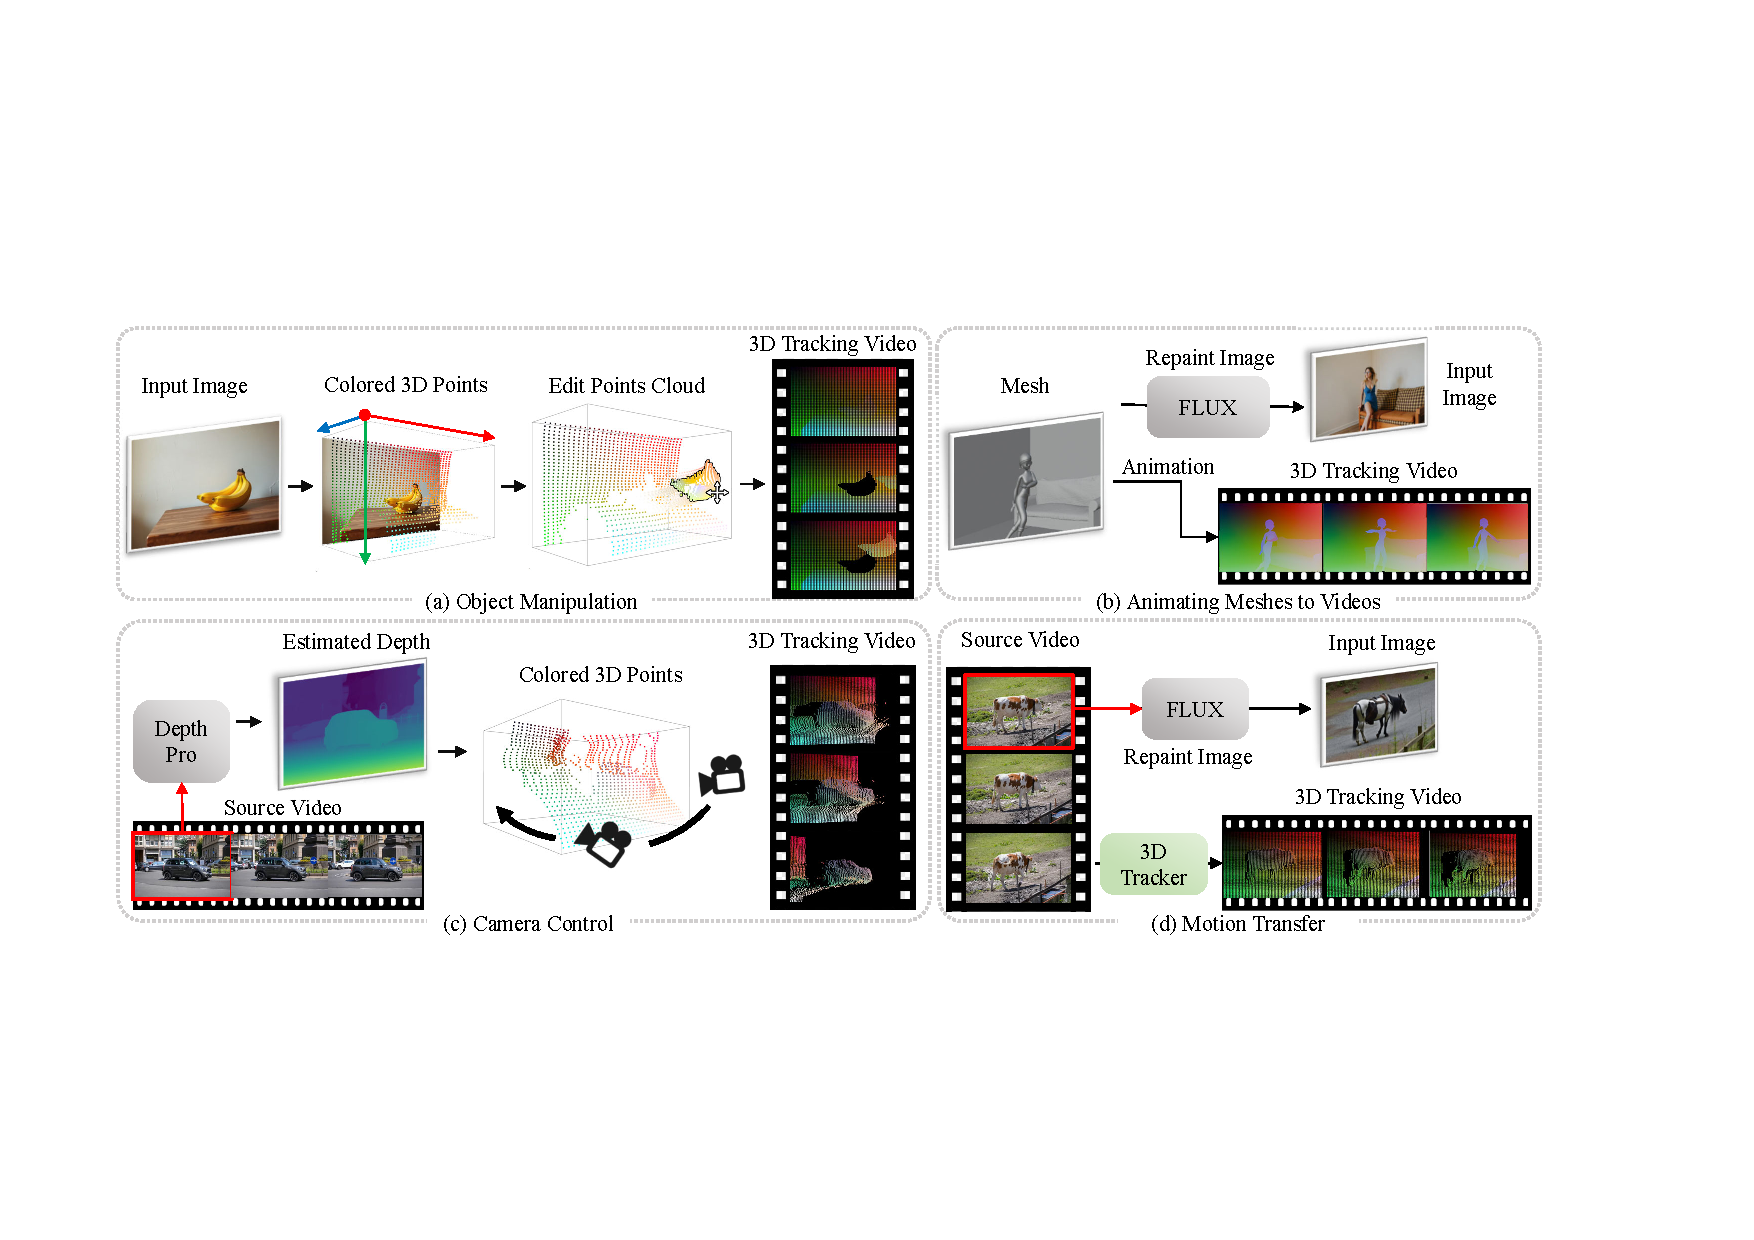
\includegraphics[width=\textwidth]{pictures/4taskpipe.pdf}
    \caption{\textbf{3D tracking video generation} in (a) object manipulation, (b) animating mesh to video generation, (c) camera control, and (d) motion transfer.}
    \label{fig:pipe-tasks}
\end{figure*}
\subsection{Finetuning with 3D tracking videos}
\label{sec:tracking}

We add a 3D tracking video as an additional condition to our video diffusion model. As shown in Figure~\ref{fig:pipe} (a, b), the 3D tracking video is rendered from a set of moving 3D points $\{\mathbf{p}_i(t)\in\mathbb{R}^3\}$, where $t=1,...,T$ means the frame index in the video. The colors of these points are determined by their coordinates in the first frame, where we normalize the coordinates into $[0,1]^3$ and convert the coordinates into RGB colors $\{\mathbf{c}_i\}$. 
Note we adopt the reciprocal of z-coordinate in the normalization.
These colors remain the same for different timesteps $t$. Then, to get a specific $t$-th frame of the tracking video, we project these 3D points onto the $t$-th camera to render this frame. In Sec.~\ref{sec:control}, we will discuss how to get these moving 3D points and the camera poses of different frames for different control tasks. Next, we first introduce the architecture to utilize the 3D tracking video as a condition for video generation.

\textbf{Injecting 3D tracking control}. We follow a similar design as the ControlNet~\cite{zhang2023adding,chen2025pixart} in \methodname to add the 3D tracking video as the additional condition. As shown in Figure~\ref{fig:pipe} (d), we apply the pretrained VAE encoder to encode the 3D tracking video to get the latent vector. Then, we make a trainable copy of the pretrained denoising DiT, called condition DiT, to process the latent vector of the 3D tracking video. The denoising DiT contains 42 blocks and we copy the first 18 blocks as the condition DiT. In the condition DiT, we extract the output feature of each DiT block, process it with a zero-initialized linear layer, and add the feature to the corresponding feature map of the denoising DiT. We finetune the condition DiT with the diffusion losses while freezing the pretrained denoising DiT. 
% \ly{todo: add more details in this part, to be more precise.}

% \textbf{Discussion: dense or sparse 3D points}. Dense 3D tracking points allow

\textbf{Finetuning details}.
To train the \methodname model, we construct a training dataset containing both real-world videos and synthetic rendered videos. The real-world videos are from MiraData~\cite{ju2024miradatalargescalevideodataset} while we use the meshes and motion sequences from Mixamo to render synthetic videos. All videos are center-cropped and resized to $720 \times 480$ resolution with 49 frames. 
We only finetune the copied condition DiT while freezing all the original denoising DiT.
To construct the 3D tracking video for the rendered videos, since we have access to the ground-truth 3D meshes and camera poses for the synthetic videos, we construct our 3D tracking videos directly using these dense ground-truth 3D points, which results in dense 3D point tracking. For real-world videos, we adopt SpatialTracker~\cite{xiao2024spatialtracker} to detect 3D points and their trajectories in the 3D space. Specifically, for each real-world video, we detect 4,900 3D evenly distributed points and track their trajectories. For training, we employ a learning rate of $1\times 10^{-4}$ \ using the AdamW optimizer. We train the model for 2000 steps using the gradient accumulation strategy to get an effective batch size of 64. The training takes 3 days on 8 H800 GPUs. 




\subsection{Video generation control}
\label{sec:control}
In this section, we describe how to utilize \methodname for the following controllable video generation.

\subsubsection{Object manipulation}
\methodname can generate a video to manipulate a specific object. As shown in Figure~\ref{fig:pipe-tasks} (a), given an image, we estimate the depth map using Depth Pro~\cite{bochkovskii2024depth} or MoGE~\cite{wang2024mogeunlockingaccuratemonocular} and segment out the object using SAM~\cite{kirillov2023segment}. Then, we are able to manipulate the point cloud of the object to construct a 3D tracking video for object manipulation video generation.

\begin{figure*}[h]
    \centering
    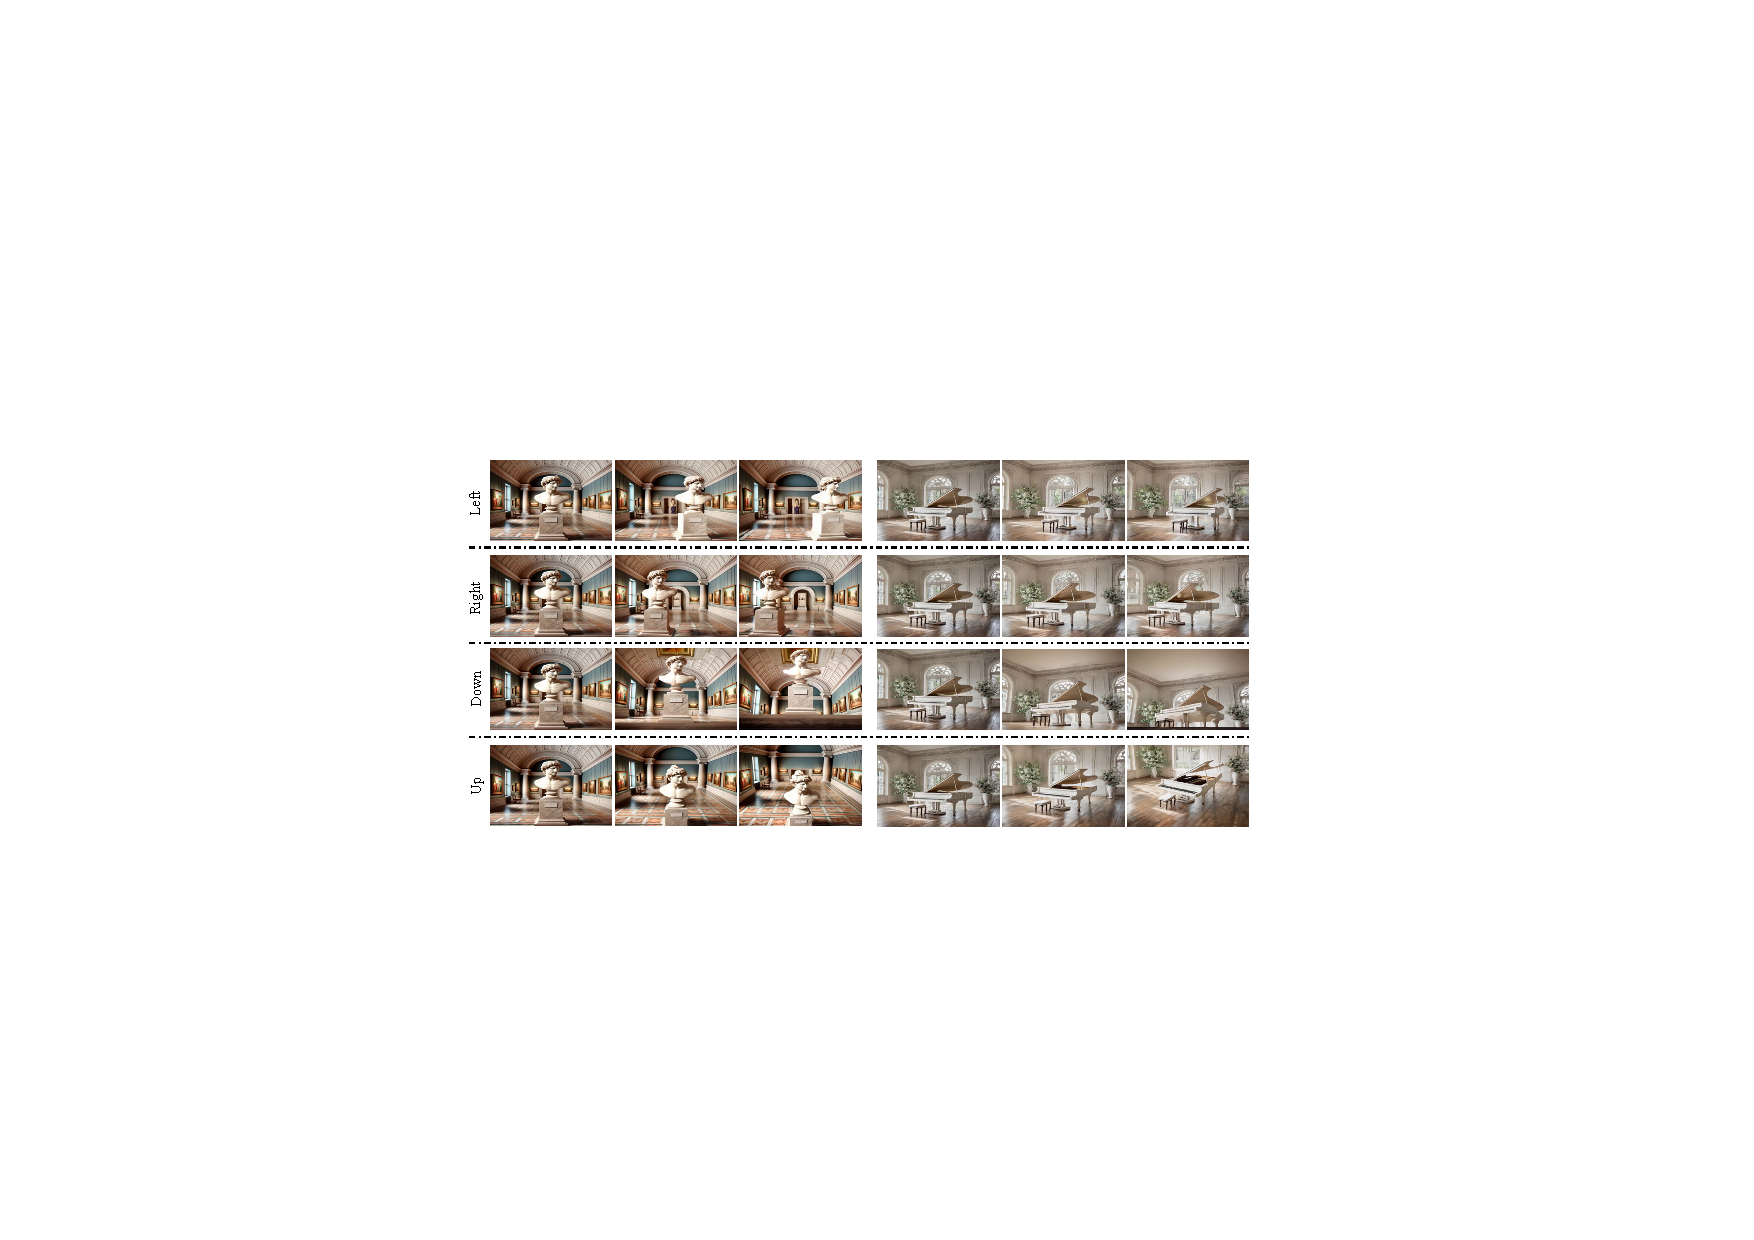
\includegraphics[width=\textwidth]{pictures/cam1.pdf}
    \caption{\textbf{Qualitative results of \methodname on the camera control task}. We show 4 trajectories (left, right, up, down) with large movements.}
    \label{fig:camctrl}
\end{figure*}

\subsubsection{Animating meshes to videos}
\methodname enables the creation of visually appealing, high-quality videos from simple animated meshes. While many Computer Graphics (CG) software tools provide basic 3D models and motion templates to generate animated meshes, these outputs are often simplistic and lack the detailed appearance and geometry needed for high-quality animations. Starting with these simple animated meshes, as shown in Figure~\ref{fig:pipe-tasks} (b), we generate an initial visually appealing frame using a depth-to-image FLUX model~\cite{flux}. We then produce 3D tracking videos from the animated meshes, which, when combined with the generated first frame, guide \methodname to transform the basic meshes into visually rich and appealing videos.

% \subsubsection{Physically-aware video generation}
% Current video generation methods~\cite{yang2024cogvideox,keling,opensora,kong2024hunyuanvideo} often fail to produce physically plausible videos because their diffusion models operate solely in the pixel space, lacking any 3D awareness. In contrast, \methodname leverages 3D tracking videos as guidance, incorporating 3D cues to ensure the generated videos are physically plausible. To achieve this, we utilize Blender's physics engine to create animated meshes, which are then used to produce 3D tracking videos following Figure~\ref{fig:pipe-tasks} (b), enabling \methodname to generate videos with more physical plausibility.

\subsubsection{Camera control}
Previous approaches~\cite{he2024cameractrl,wang2024motionctrl} rely on camera or ray embeddings as conditions to control the camera trajectory in video generation. However, these embeddings lack true 3D awareness, leaving the diffusion models to infer the scene's 3D structure and simulate camera movement. In contrast, \methodname significantly enhances 3D awareness by incorporating 3D tracking videos for precise camera control. To generate videos with a specific camera trajectory, as shown in Figure~\ref{fig:pipe-tasks} (c), we first estimate the depth map of the initial frame using Depth Pro~\cite{bochkovskii2024depth} and convert it into colored 3D points. These points are then projected onto the given camera trajectory, constructing a 3D tracking video that enables \methodname to control camera movements with high 3D accuracy.


\subsubsection{Motion transfer}
As shown in Figure~\ref{fig:pipe-tasks} (d), \methodname also facilitates creating a new video by transferring motion from an existing source video. First, we estimate the depth map of the source video’s first frame and apply the depth-to-image FLUX model~\cite{flux} to repaint the frame into a target appearance guided by text prompts. Then, using SpatialTracker~\cite{xiao2024spatialtracker}, we generate a 3D tracking video from the source video to serve as control signals. Finally, the \methodname model generates the target video by combining the edited first frame with the 3D tracking video.

